\documentclass{blue-book}
\NoteNumber{3}

\usepackage{graphicx}
\usepackage{amssymb,amsmath}
\usepackage{listings}

\let\sometime=\lozenge
\let\always=\Box

\title{Explanations for Forward-Chaining Rules-Based Systems (to be implemented in Prolog)}
\author{Louise A. Dennis}

\begin{document}
\maketitle
I've been thinking about explanations for deductions made in rules-based reasoning systems.  This represents a first pass with a focus on producing a simple algorithm but one which hopefully has the right structure for improvements.  I'm designing the pseudo-code and data structures around the concept of implementation within a logic programming based language, such as Prolog, because of the ease of representing logical formulae in such languages.

\section{Rules, Facts and Deductions}

\begin{description}
\item[Facts] Facts are statements that the system either knows at the start of reasoning (provided as part of an initial problem statement) or have been deduced during the course of reasoning.  Facts are represented as ground first order formulae - e.g. \texttt{name(mary)}, \texttt{age(34)}.
\item[Rules] Rules are used to deduce new facts from old facts.  They are represented as $A \rightarrow B$ which means that if $A$ is known then $B$ may be deduced.  For the present I will assume that $B$ is a single literal and $A$ is a list of literals representing a conjunction.  We can $A$ the antecedants and $B$ the consequent.  Literals appearing in rules may not be ground.  The following are correctly formed rules:
\begin{eqnarray}
[residence(mary, City), inuk(City)] & \rightarrow & inuk(mary). \\ 
{}[name(Name), residence(Name, City), inuk(City)]  & \rightarrow & inuk(Name).
\end{eqnarray}
I'm using Prolog style notation so atoms starting with capital letters are variables that will be instantiated when the rule is applied and those starting with lower case letters are constants.  So the first rule here says that ``if mary lives in City and City is in the UK then mary lives in the uk".  The second more generally says that ``if someone's name is Name and Name lives in City and City is in the uk then Name lives in the uk".

If we had the facts \texttt{name(mary)}, \texttt{residence(mary, manchester)} and \texttt{inuk(manchester)}.  Then we would expect to be able to deduce a new fact \texttt{inuk(mary)} using either of these rules.
\end{description}

\section{A Data Structure for Deductions}
I am going to represent deductions as a directed acyclic graph.  The nodes in a graph consist of a fact and a label -- the label is either \texttt{initial\_fact} (indicating that the fact is one of the initial inputs) or an ID for a rule.  Two nodes, $n_1$ and $n_2$ are connected by an edge, $n_1 \rightarrow n_2$ if the fact labelling $n_2$ is one of the antecedants for the rule labelling $n_1$.  At some point we will need some well-formedness definitions for these graphs but, for the time being, I'll simply assume that we are always talking about ones that are, in some sense, sensible and rational.  So, for instance the DAG in figure~\ref{fig:dag} shows how rule (2) above deduced \texttt{inuk(mary)} from the initial facts.
\begin{figure}[htb]
\begin{center}
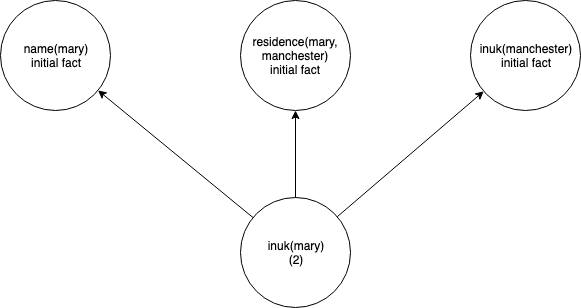
\includegraphics[width=0.6\textwidth]{images/bb3_dag.png}
\end{center}
\caption{A Directed Acyclic Graph representing a deduction}
\label{fig:dag}
\end{figure}

\section{Construction DAGs using Forward Chaining}
When performing deduction in rules-based systems you can use either forward or backward chaining.  I think a Deduction DAG can be constructed using either method but to start with we will look just at forward chaining.  The input to the algorithm is a fact that the user wishes to establish.  The algorithm tries the rules repeatedly adding new facts until the desired fact is established or no new facts can be deduced.  All nodes and rules are given unique IDs (for instance by simply counting up through the numbers).  I'm representing nodes as \texttt{node(ID, F, L, NodeList)} where \texttt{ID} is the id number of node, \texttt{F} is the node fact, \texttt{L} is the rule ID or \texttt{initial\_fact} label of the node and \texttt{NodeList} is the list of nodes this node is connected to in the DAG (i.e., the antecedants of the rule).

First we initialise our problem.  I'm using \texttt{assert} like Prolog assert -- so assert creates new data to be used in reasoning

\begin{verbatim}
INITALISE_PROBLEM:
   INPUT: set of facts: F, set of rules R
   FOREACH f in F:
      ID_n = new ID
      assert(node(ID_n, f, initial_fact, []))
   FOREACH A -> B in R:
      ID_r = new ID
      assert(rule(ID_r, A, B)) 
\end{verbatim}

Next we have a rule for seeing if we can deduce some fact.  We refer to this fact as a query.  A query is a literal (e.g., \texttt{inuk(mary)}, $\lnot$ \texttt{inuk(mary)}, \texttt{inuk(X)}). Where the first of these asks whether mary is in the uk, the second whether mary is not in the uk and the third whether someone, X, is in the UK -- in this last case we would expect the algorithm to return a value for X.

We start with what happens when we want to deduce something that has been established as fact (so appears as a node in our DAG).

\begin{verbatim}
deduce(Q, node(ID, Q, DAG)):-
   node(ID, Q, DAG)
\end{verbatim}
I'm writing the above more or less as Prolog Code so, for instance, if we have \texttt{node(20, name(mary), initial\_fact, [])} asserted as part of our problem statement then a call to

\begin{verbatim}
?- deduce(name(mary), DAG).
\end{verbatim}
in the Prolog interpreter will return

\begin{verbatim}
DAG = node(20, name(mary), initial_fact, []))
\end{verbatim}

And a call to 
\begin{verbatim}
?- deduce(name(X), DAG).
\end{verbatim}
in the Prolog interpreter will return

\begin{verbatim}
X = mary
DAG = node(20, name(mary), initial_fact, []))
\end{verbatim}

Next we look at how we might deduce a new fact.

\begin{verbatim}
deduce(Q, DAG):-
   rule(ID_r, A, B),
   check_antecedants(A, NodeList),
   \+ node(ID, B, _)
   ID_n = new ID,
   assert(node(ID_n, ID_r, NodeList)),
   deduce(Q, DAG)
	
check_antecedants([],[]).
check_antecedants([H|T], [node(ID, H, DAG)|NodeList]):-
   node(ID, H, DAG),
   check_antecedants(T, NodeList).
\end{verbatim}
What is happening here is that we pick a rule and we see if all the antecedants of the rule are facts using \texttt{check\_antecedants/2} (in Prolog this will also instantiate variables where relevant).  We then check that the consequent of the rule, $B$, is not already a fact (given the instantiations of any variables), if not we assert a new node and then try, once more, to establish Q.  Since we are thinking in terms of Prolog, this will automatically backtrack and pick a different rule to try if either all the antecedants are not facts or if the consequent is already established.
	
\texttt{check\_antecedants} recurses through the list of antecedants to see if they are all facts, if they are it adds the relevant nodes to a list which it returns.


If we were to run this algorithm on the input \texttt{deduce(inuk(mary), DAG)} where we had the nodes: 
\begin{itemize}
\item \texttt{node(1, name(mary), initial\_fact)}, 
\item \texttt{node(2, residence(mary, manchester), initial\_fact)}, 
\item \texttt{node(3, inuk(manchester), initial\_fact)} 
\end{itemize} and the rule \texttt{rule(1, [name(N), residence(N, C), inuk(C)], inuk(N)} we should get the output

\begin{verbatim}
?- deduce(inuk(mary), DAG).

DAG = node(4, inuk(mary), 1, [node(1, name(mary), initial_fact), 
                        node(2, residence(mary, manchester), initial_fact), 
                        node(3, inuk(manchester), initial_fact)]).
\end{verbatim}

\section{Explanation}

Now we look at how we can construct an explanation given a DAG representing a deduction.

Since we anticipate wanting to use dialogues for explanation we will assume that only an explanation for one deductive step is required (we can probably extend this later).  So actually our algorithm is pretty simple.


\begin{verbatim}
explain(N, "F is an initial fact"):-
   node(N, F, initial_fact, []).
explain(N, "F follows from the rule that states that A implies F and all the A were true"):-
   node(N, F, RULE_ID, NodeList),
   rule(RULE_ID, A, F).
\end{verbatim}

\section{Discussion}
My Prolog is pretty rusty so I suspect some work may be needed to translate this into working code (particularly the generation of ID numbers and the construction of strings from the output).  I think in the explanation algorithm we may also need to do some work to instantiate $A$ properly.

Moving on, once we can explain one node in a one step way in a DAG, then a user can drill down further to question, for instance, why the $A$ are true (we may need to tag each A with their node number here so the user can identify the node in the DAG that established each antecedant).

We will also need to think, in future about how a user can ask why something isn't true which is a more complex explanation problem (in~\cite{DennisAAMAS21} we do this by having the system ask them why they thought  something should be true and then trying to narrow down to the source of disagreement).

We should check if we can build DAGs using backward chaining as well as forward chaining (I think we can).

In future work we want to look at nodes where facts are established because of a recommendation algorithm rather than being initial facts or rule based deductions.

\bibliography{bluebook}
\bibliographystyle{apalike}


\end{document}